%\documentclass[11pt,a4paper]{article}
\usepackage[utf8]{inputenc}
\usepackage[dutch]{babel}
\usepackage{pgfplots}
\usepgfplotslibrary{units}
\usepackage{float}
\usepackage{amsmath,amsthm}
\usepackage{amsfonts}
\usepackage{amssymb}
\usepackage[left=2cm,right=2cm,top=2.5cm,bottom=2cm]{geometry}
\usepackage{graphicx}
\usepackage{multicol}
\usepackage{enumerate}
\usepackage{fancyhdr}
\pagestyle{fancy}
\usepackage{algorithm}
\usepackage{algpseudocode}
\usepackage{pgfplots}
\usepackage{multirow}
\usepackage{tikz}
\usetikzlibrary{calc}

\floatname{algorithm}{Algoritme}


\usepackage[font=small,labelfont=bf]{caption}
\captionsetup[table]{aboveskip=-0.8em}
\captionsetup[table]{belowskip=-0.7pt}


\lhead {DAIII Project: punten plaatsen} 
\chead{BAZ(~ \thepage ~ )NGA} 
\rhead{Robbert Gurdeep Singh}


\cfoot{} % get rid of the page number 

\usepackage{hyperref}
\usepackage{chngcntr}
\counterwithin*{section}{part}
\counterwithin{algorithm}{section}
\counterwithin{table}{section}
\counterwithin{figure}{section}

\hypersetup{
    colorlinks=false,
    pdfborder={0 0 0},
}

\author{Robbert Gurdeep Singh}
\title{{Project Algoritmen en datastructuren III}\\ \Huge Genetische algoritmen}
%\date{}



\pgfplotsset{compat=1.8}


\newcommand{\drawGraph}[4]{
\begin{tikzpicture}
\begin{axis}[scale only axis, 
	%x-as	
    xmin=0,
	xlabel=#1,	
	%y-as
	ylabel=#2,
	ymin=0,
	%Style
	height=5em,width=.37\textwidth,
	enlargelimits=0.05,
	grid=major,	legend pos=south east
]
#3
\end{axis}
\end{tikzpicture}
}


\newcommand{\lxaxis}[3]{\begin{tikzpicture}
\begin{axis}[scale only axis, 
cycle list name=exotic,
    xmode=log,
    log ticks with fixed point,
	%x-as	
	xlabel=#2,	
	%y-as
	ylabel=#1,
	ymin=0,
	%Style
	height=5em,width=.37\textwidth,
	enlargelimits=0.05,
	grid=major,	legend pos=south east
]
#3

\end{axis}
\end{tikzpicture}}

\newcommand{\rlxaxis}[3]{\begin{tikzpicture}
\begin{axis}[scale only axis, 
cycle list name=exotic,
    xmode=log,
    log ticks with fixed point,
	%x-as	
	xlabel=#2,	
	%y-as
	ylabel=#1,
	%Style
	height=5em,width=.37\textwidth,
	enlargelimits=0.05,
	grid=major,	legend pos=south east
]
#3

\end{axis}
\end{tikzpicture}}

\newcommand{\nxaxis}[3]{\begin{tikzpicture}
\begin{axis}[scale only axis,
cycle list name=exotic, 
	%x-as	
    xmin=0,
	xlabel=#2,	
	%y-as
	ylabel=#1,
	ymin=0,
	%Style
	height=5em,width=.37\textwidth,
	enlargelimits=0.05,
	grid=major,	legend pos=south east
]
#3

\end{axis}
\end{tikzpicture}}


\newcommand{\rnxaxis}[3]{\begin{tikzpicture}
\begin{axis}[scale only axis, 
cycle list name=exotic,
	%x-as	
    xmin=0,
	xlabel=#2,	
	%y-as
	ylabel=#1,
	%Style
	height=5em,width=.37\textwidth,
	enlargelimits=0.05,
	grid=major,	legend pos=south east
]
#3

\end{axis}
\end{tikzpicture}}

\newcommand{\itemMB}[1]{
	\item[$\boldsymbol{#1}$:]
}




\newcommand{\abs}[1]{
	\lvert #1 \rvert
}

\newcommand{\addploti}[1]{\addplot table [y=i, x=testValue, col sep=comma] {../../tests/param_results/#1.log};}
\newcommand{\addplotf}[1]{\addplot table [y=f, x=testValue, col sep=comma] {../../tests/param_results/#1.log};}
\newcommand{\addplott}[1]{\addplot table [y=t, x=testValue, col sep=comma] {../../tests/param_results/#1.log};}

\definecolor{mymark}{HTML}{EBB8B8}

\begin{document}

\twocolumn[\begin{@twocolumnfalse}
    \maketitle
\end{@twocolumnfalse}]
\subsection{Selectie Paren}
\label{sub:SUS}
In het genetisch algoritme moeten er individuen worden geselecteerd die seks zullen hebben ter vorming van nieuwe individuen.
Tijdens deze selectie moeten we er op letten dat dat we niet enkel de fitste individuen kiezen. De kans is namelijk reëel dat de genetische informatie van een ``slecht'' individu aanleiding kan geven tot een zeer goed individu na paren. Natuurlijk willen we diegenen met een hogere fitheid wel een grotere kans geven zich voort te planten.

\subsubsection{Idee}
Stellen we onze individuen voor als blokjes met een grootte die evenredig is met hun fitheid, dan kunnen we ze na elkaar plaatsen en iets bekomen als in figuur \ref{fig:SUS}. 
We kunnen dan ergens starten en met gelijke stappen vooruitgaan. Bij elke stap nemen we het stuk waar we bijstaan. Zo is de kans dat een stuk gekozen wordt recht evenredig met zijn fitness. Deze aanpak wordt Stochastic Universal Sampeling genoemd.
%todo

\begin{center}
\begin{figure}[H]
\centering
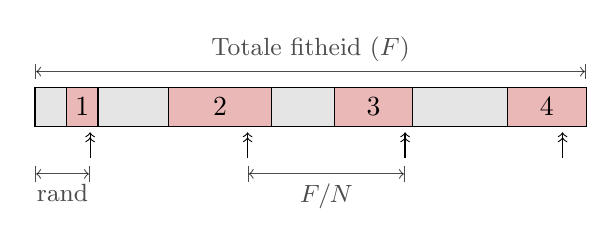
\begin{tikzpicture}

\foreach \x in {0.7,2.7,4.7,6.7}
    \draw[->>] (\x cm,-0.4cm) -- (\x cm,-2pt);

\draw[fill=black,fill opacity=0.1] (0,0) rectangle (7,0.5);

\foreach \x in {0.4,0.8,1.7,3,3.8,4.8,6}
    \draw (\x cm,0pt) -- (\x cm,0.5);

\draw[fill=mymark] (0.4,0) rectangle node {1} (0.8,0.5);
\draw[fill=mymark] (1.7,0) rectangle node {2} (3.0,0.5);
\draw[fill=mymark] (3.8,0) rectangle node {3} (4.8,0.5);
\draw[fill=mymark] (6.0,0) rectangle node {4} (7.0,0.5);

\draw[|<->|,black,opacity=0.7] (0,0.7) -- node[above] {\small Totale fitheid ($F$)} (7,0.7);
\draw[|<->|,black,opacity=0.7] (2.7,-0.6) -- node[below] {\small $F/N$} (4.7,-0.6);
\draw[|<->|,black,opacity=0.7] (0,-0.6) -- node[below] {\small rand} (0.7,-0.6);

%node[anchor=north] {\x};
\end{tikzpicture}
\caption{Visualisatie Stochastic Universal Sampling}
\label{fig:SUS}
\end{figure}
\end{center}


\subsubsection{Algoritme}
Het algoritme die het voorgaande idee implementeert heeft volgende vorm:
	\begin{algorithm}[H]
	 	\caption{Stochastic Universal Sampeling}
		\begin{algorithmic}
		\Require 
			\State $P$, te grote lijst van individuën 
			\State $N_l$, gewenste aantal individuen
		\Ensure returnt een lijst van gekozen individuen
		\Function{SUS}{$P$,$N_t$}
		\State Q $\gets \emptyset$
		\State total $\gets \sum_{x \in P} f(x)$ 
		\State size $\gets \frac{\text{total}}{N_l}$
		\State offset $\gets$ arbitraire waarde uit $\left\lbrack 0,\text{size} \right\rbrack$
		\State $t \gets$ offset
		\For{\textbf{each} $p \in P$} 
		\State $t = t-p.$fitness
		\If{$t<0$}
			\State $Q = Q \cup \lbrace p \rbrace$
			\State $t = t+$offset
		\EndIf
		\EndFor		
		\State \Return i
		\EndFunction

		
		\end{algorithmic}
		\label{alg:SUS}
	\end{algorithm}		
% subsubsection  (end)

\subsubsection{Complexiteit}
\label{ssub:SUSComplexity}
We moeten nagenoeg alle individuen in de populatie overopen. We kunnen dus stellen dat de complexiteit $ \Theta(\abs{P})$ is, met $\abs{P}$ de grootte van de populatie. Nu is $\abs{P}$ geen argument van ons programma. Dus bekomen we een complexiteit van \[T(n) = \Theta(1)\]
% subsubsection  (end)

\subsubsection{Alternatief}
\label{sec:positiveTournament}
Een alternatief bestaat er in tournament selcetion te gebruiken zoals in Algoritme~\ref{alg:tournament} uit sectie~\ref{sub:tournament}. Hierbij moeten we natuurlijk wel groter dan gebruiken in plaats van kleiner dan om meer kans te geven aan betere individuen. De complexiteit hiervan is  \[T(n) = \Theta(\abs{P} \cdot P_M) = \Theta(1)\]

%\section{Bronnen}
Er moet vermeld worden dat het \texttt{icosagon.poly} bestand afkomstig is van Jonathan Peck. We hebben dit bestand uitgewisseld om een andere figuur dan het gegeven vierkant te hebben samen met een notie van de maximale fitheid voor 50 punten in deze figuur. Code is er natuurlijk niet uitgewisseld.

\begin{thebibliography}{9}

\bibitem{lamport94}
  Haupt, Randy L., and Sue Ellen Haupt. ``Practical genetic algorithms.'' (2004).

\bibitem{baker85}
Baker, James Edward. "Adaptive selection methods for genetic algorithms." Proceedings of an International Conference on Genetic Algorithms and their applications. 1985.

\bibitem{parra9748125}
Pit, Laurens Jan. "Parallel genetic algorithms." MS (Computer Sci.) Dissertation (1995).

\bibitem{cuofiezafm}
Brinkmann, Gunnar. "Datastructuren en Algoritmen III, 2014." Cursus (2014)

\bibitem{MPIDOC}
University of Tennessee, "MPI: A Message-Passing Interface Standard" Online PDF. http://www.mpi-forum.org/docs/mpi-3.0/mpi30-report.pdf (2012)



\end{thebibliography}
\end{document}